% 第 15 章  TFT 中的状态与可观测量
% 原文：Chapter 15: States and observables in TFT（pp. 251–264，印刷页码 250–263）
% 第 34 讲；2021 年 8 月 13 日
% ============================================================================
\chapter{TFT 中的状态与可观测量}\label{ch:15}

\begin{flushright}\small 第 34 讲；2021 年 8 月 13 日\end{flushright}

\begin{keytakeaways}
本章用导出代数几何的眼光重新审视拓扑场论（TFT）中的状态与可观测量。对 $n$ 维 TFT $\cZ$，局部算子构成 $\mathbb{E}_n$-代数 $\cZ(S^{n-1})$（Dunn--Lurie 可加性：$\mathbb{E}_n=\mathbb{E}_k+\mathbb{E}_\ell$，$k+\ell=n$）；其同调是 $\mathbb{P}_n$-代数，取 $\Spec$ 得到 $n$-移位 Poisson 簇——真空模空间 $\cM^0$。由此，形变量子化把 $\cM^0$ 还原为 $\mathbb{E}_n$-代数（即可观测量），而几何量子化则给出状态空间。当理论来自一个 $n$-移位辛流形 $\cM$ 时，对 $k$ 维时空 $M$，$\mathrm{Map}(M,\cM)$ 是 $(n-k)$-移位辛的：其形变量子化给出 $M$ 上的可观测量（因子化同调 $\int_M\cZ(S^{n-1})$），其几何量子化给出 $M$ 上的状态空间。本章后半以二维 $B$-模型为例具体展开：$B_X(\mathrm{pt})=D^b\mathrm{Coh}(X)$，局部算子为 $\mathrm{HH}^*(X)$，$\cM^0=T^*X[1]$；据此讨论凝聚层的奇异支撑、Atiyah 类，以及局部完全交（lci）空间上多出来的“翅膀”。最后回到几何 Langlands 的 $B$-侧：$\Loc_{G^\vee}(C)$ 是 lci，故其上的层具有良好定义的奇异支撑。
\end{keytakeaways}

回想我们一直在探讨一个总体想法：我们研究的是 TFT 的导出代数几何。也就是说，我们从一个 TFT 出发，从中提取大量结构。例如，我们可以提取局部算子之环，并且发现它甚至是交换的。现在我们要在导出情形下重新审视这一点。在导出情形下，算子并不真正交换，它们构成的是 $\mathbb{E}_n$-代数。也就是说，若 $\cZ$ 是一个 $n$ 维 TFT，则 $\cZ(S^{n-1})$ 是 $\mathbb{E}_n$-代数。

关于 $\mathbb{E}_n$-代数，最重要的知识是 Dunn--Lurie 可加性。它大致是说：一个 $\mathbb{E}_n$ 结构的数据等价于 $n$ 个相容的 $\mathbb{E}_1$ 结构的数据。也就是说，在 operad 的层面有
\begin{equation}\tag{15.1}
\mathbb{E}_n=\mathbb{E}_k+\mathbb{E}_\ell
\end{equation}
（其中 $k+\ell=n$）。% [Tutor Note: Dunn--Lurie 可加性通常表述为 $\mathbb{E}_m\otimes\mathbb{E}_n\simeq\mathbb{E}_{m+n}$，其几何含义是“$n$ 维小圆盘可以沿 $n$ 个彼此独立的方向分解”；这里作者写成 $\mathbb{E}_n=\mathbb{E}_k+\mathbb{E}_\ell$ 是简写，不要误读为直和。]

我们还指出了几何上的一点：$\mathbb{E}_n$-代数的上同调\footnote{对我们而言，$\mathbb{E}_n$-代数就是一个上链复形，其运算是这些“小圆盘”相互碰撞给出的。当我们说上同调时，只是把上链复形取上同调。在上同调的层面上，Poisson 括号的做法是：取某点处的一个算子，并在它周围的小球面上积分。}是一个 $\mathbb{P}_n$-代数。$\mathbb{P}_n$-代数是指带有次数为 $1-n$ 的括号 $\{,\}$ 的交换代数。当 $n$ 为奇数时，$\mathbb{P}_n$-代数的行为像普通的 Poisson 代数，只不过一切都带分次，且括号 $\{,\}$ 的次数非零。当 $n$ 为偶数时，$\mathbb{P}_n$-代数是 Gerstenhaber 代数，此时符号约定不同：它是 Poisson 的某种“超”版本。

现在我们要看看能从其中榨出多少代数几何。我们已经谈过很多如何从算子的结构中榨出代数几何，但那是通常的（交换）代数几何；现在我们想得到某种辛几何。

换一种说法：我们希望理解 TFT 中的状态与可观测量。状态经由形变量子化产生，可观测量经由几何量子化产生；因此等价地，我们希望在一般 TFT 的框架下理解形变量子化与几何量子化。

% ============================================================================
\section{几何量子化与形变量子化}
\begin{sectionkey}
本节回顾量子力学中“状态空间”与“可观测量代数”的二分，并把它对应到形变量子化（从相空间造出算子代数）与几何量子化（从相空间造出状态空间）。要点有二：形变量子化是统一、典范的构造，其一阶微小扰动由 Poisson 括号给出；几何量子化则依赖于极化等额外选择，但物理上应与极化无关，这由 Fourier 变换与半密度（以及相关的自旋结构）等现象体现。
\end{sectionkey}

这是一个可以讲整整一门课的主题。我们只想突出其中的关键特征。

考虑量子力学，即一维量子场论。量子力学中有两个主要角色：
\begin{itemize}
  \item 状态构成的 Hilbert 空间 $\cH$，以及
  \item 可观测量构成的结合代数 $A$。
\end{itemize}
实际上我们要考虑的是纯态，即这个空间中的射线。状态空间是一维理论在一点上的取值：
\begin{equation}\tag{15.2}
\mathrm{QM}(\mathrm{pt})=\cH.
\end{equation}
可观测量的结合代数 $A$ 作用在 $\cH$ 上。因此总起来说，这由一个代数与一个模构成：
\begin{equation}\tag{15.3}
A\ \circlearrowleft\ \cH.
\end{equation}
量子力学中的一切都用这些来表述。用 $\QC$ 的语言说：
\begin{equation}\tag{15.4}
\QC(\mathrm{pt}\sqcup\mathrm{pt})=\End(\cH).
\end{equation}
我们可以把这两个点看作一维时空中某个奇点的链环（link）。所以它们正是我们一直在发展的局部算子。

我们通过经典力学的量子化得到量子力学。对我们而言，一个（非退化\footnote{如果我们改而考虑（更大的）Poisson 流形类，那么对应的就是可能退化的经典力学系统。}的）经典力学系统由辛流形 $M$ 刻画，这就是系统的相空间。于是量子化是这样一种程序：输入 $M$，输出状态空间 $\cH$ 与可观测量代数 $A$，使得 $A\ \circlearrowleft\ \cH$。\term{形变量子化}{deformation quantization}是从 $M$ 构造可观测量（$A$）的过程；\term{几何量子化}{geometric quantization}是从 $M$ 构造状态（$\cH$）的过程。

\begin{srcrem}{102}
人们有时说，形变量子化是一门科学（至少是一个函子），而几何量子化更像是一门艺术。
\end{srcrem}

\subsection{形变量子化}

设 $M$ 是辛流形。则函数环
\begin{equation}\tag{15.5}
A_0=(\cO(M),\{-\})
\end{equation}
自然地是一个 Poisson 代数。给定一个 Poisson 代数，我们可以要求它在 $h$ 中的一个形变 $A_h$，即一族以 $h$ 为参数、满足下述条件的结合代数：
\begin{equation}\tag{15.6}
A_h|_{h=0}\simeq A_0
\end{equation}
是交换的，并且
\begin{equation}\tag{15.7}
\frac{d}{dh}[-]=\{-\}.
\end{equation}
% [Tutor Note: 原文（以及抽取文本）中这个形变参数有时被写成 $\hbar$，但页面图 (15.6)--(15.9) 上明确用的是斜体 $h$，不是 $\hbar$。本译本按页面图统一用 $h$；这不是把 $h$ 与 Planck 常数 $\hbar$ 混同，而是笔记作者的记号。]

也就是说，我们是在说下面这件事。给定 $a_0,b_0\in A_0$，选取提升
\begin{equation}\tag{15.8}
a,b\in A_h,
\end{equation}
于是 $[a,b]$ 被 $h$ 整除，即在 $0$ 处为零。那么我们说 Poisson 括号由下式给出：
\begin{equation}\tag{15.9}
\{a_0,b_0\}=\frac{[a,b]}{ih}\bmod h.
\end{equation}

\begin{srcrem}{103}
这个想法是：在结合代数的世界里，Poisson 代数构成交换代数的“切空间”；把一个交换代数形变为结合代数的一阶数据，就是 Poisson 括号。
\end{srcrem}

事实证明，每个 Poisson 代数都有形变量子化，并且所有形变可以用某种方式参数化。这些形变量子化的集合看起来就像 Poisson 世界内部的形变（后者有明确的同调描述）。但实际上存在一个典范的形变。换句话说，我们知道辛流形总可以被典范地形变量子化。Kontsevich 对一般 Poisson 代数解决了这个问题；对于辛情形，更早由 所解决。% [Tutor Note: 原文此处人名留空，页面上只有一个手写的“cite”批注框，显系作者尚未补上引用。按数学史，辛流形形变量子化的早期工作应指 Fedosov（以及更早的 Weyl--Wigner--Moyal 传统）；译者不擅自替正文补入人名，请读者据此对照文献。]

\subsection{几何量子化}

形变量子化是一个非常具体的构造。几何量子化的定义则粗略一些。

现在我们要找状态空间：形变量子化之上的一个模。它应当是一个非常小的模，例如不可约模，即某种“最小的非零模”。有许多愿望清单，我们不打算深入；但要点是，几何量子化大致就是“$M$ 的一半变量上的函数”。

\begin{srcex}{105}
考虑 $\R^n$ 中的一个粒子。系统的相空间是 $T^*\R^n$，即给定的辛流形。几何量子化为
\begin{equation}\tag{15.10}
L^2(\R^n).
\end{equation}
\end{srcex}

一般地，若 $M=T^*X$（或者若 $M$ 被极化），则我们可以写出一个 Hilbert 空间：
\begin{equation}\tag{15.11}
L^2(X).
\end{equation}
但要注意，对于“极化”（polarization）可以有很多不同的含义。% [Tutor Note: 这里作者用“极化”指实极化（把 $T_{\C}M$ 分解为全纯与反全纯两部分）；(15.11) 对应取零截面上的函数，是“实极化”的一种。后文 Example 107 说明不同极化给出的 Hilbert 空间应当同构，这正是几何量子化不依赖极化的核心诉求。]

\begin{srcex}{106}
若 $M$ 是紧 Kähler 流形（例如 $\PP^n$），则有自然的辛形式。\footnote{注意这不是全纯辛形式；Kähler 结构给出的是一个（非退化、反对称的）实 $2$-形式。}此时“一半的变量”意味着我们看的是全纯函数，即形如
\begin{equation}\tag{15.12}
\Gamma(M,\cL)
\end{equation}
的东西，其中 $\cL$ 是满足第一 Chern 类等于辛形式的线丛：$c_1(\cL)=\omega$。
\end{srcex}

\paragraph{配对}

这里有许多微妙之处。例如，$L^2(X)$ 中的元素并不是自然的函数，而是“半密度”：它们是配对之后才可以积分的东西。因此一般地，为了定义我们所关心类型的函数，需要选取体积形式丛的一个平方根。这样的选取类似于自旋结构的选取。这一切只是想说：构造几何量子化牵涉到一些选择，而这一构造是否与选择无关并非显然。

\paragraph{辛不变性}

若 $M=T^*X$，代数几何学家很容易猜测几何量子化就是 $\cO(X)$。这是一幅很糟糕的图景：几何量子化应当与极化无关。

\begin{srcex}{107}
$L^2(\R^n)$（即 $T^*\R^n$ 的几何量子化）与极化无关：对应于这一极化的 Hilbert 空间同构于对应于任何其它极化的 Hilbert 空间。例如，Fourier 变换把零截面送到 $0$ 处的纤维，并给出零截面上 $L^2$ 函数构成的 Hilbert 空间与 $0$ 处纤维上 $L^2$ 函数构成的 Hilbert 空间之间的同构。也就是说，它把“一半变量上的函数”变成“另一半变量上的函数”，并断言二者同构。
\end{srcex}

要点在于：$L^2$ 函数实际上是微局部对象，即它们在所定义空间的余切丛上具有支撑理论。它们“生活”在我们出发的整个辛空间上。所以尽管我们把该空间描述为 $L^2(\R^n)$（零截面上的函数），它其实并不依赖于极化的选取。然而 $\cO(X)$ 确实依赖于所选的极化。

把这一点讲精确的一种方式如下。给定 $\R^n$ 上的一个分布，可以赋予它一个波前集，这是 $T^*\R^n$ 的子集，由那些使该分布不再是真正函数的点与方向构成。另一样东西叫做 Wigner 分布：对任意 $f\in L^2$，我们可以把 $|f|^2$ 提升为 $T^*\R^n$ 上的一个分布。% [Tutor Note: 这里“支撑理论”与波前集、Wigner 分布之间的关系，是后文（15.51）把 $\mathrm{Ext}(\cF,\cF)$ 看成 $T^*X[1]$ 上代数的动机：$|f|^2$ 的提升就是通常的“符号”，而奇异支撑可以看作它的代数几何版本。]

% ============================================================================
\section{（拓扑）量子场论中形变量子化与几何量子化的类比}
\begin{sectionkey}
本节把“辛流形 $\to$ Poisson 代数”的对应推广为“$n$-移位辛流形 $\to$ $\mathbb{P}_n$-代数”。对 $n$ 维 TFT，局部算子 $\cZ(S^{n-1})$ 是 $\mathbb{E}_n$-代数，其真空模空间 $\cM^0=\Spec H^*\cZ(S^{n-1})$ 带有 $n$-移位 Poisson 结构；形变量子化给出 $\cZ(S^{n-1})$ 本身。因子化同调 $\int_M\cZ(S^{n-1})$ 给出 $M$ 上的可观测量，其对偶给出共形块，即状态空间。
\end{sectionkey}

主要信息是：$n$ 维量子场论（特别是对我们而言的 TFT）与所谓的 $n$-移位辛几何有类似的关系。这些移位辛流形在更高维量子场论的框架中扮演半经典相空间的角色。

\begin{srcrem}{104}
$n$-移位辛结构的定义相当晚近，见 [PTVV13]；但相关想法已经存在了一段时间，例如 Albert Schwarz 的工作。% [Tutor Note: 原文句末有手写批注“Cite”，提示作者原打算补一条文献。PTVV13 指 Pantev--Toën--Vaquié--Vezzosi 的 “Shifted symplectic structures”，是该定义的原始文献；Albert Schwarz 则更早用 odd symplectic（即 $-1$-辛）结构研究 BV 量子化。]
\end{srcrem}

回想辛流形 $M$ 给我们一个 Poisson 代数：
\begin{equation}\tag{15.13}
(\cO(M),\{-\}).
\end{equation}
类似地，我们要从移位辛流形得到类似的东西：一个 $n$-移位辛簇将是使得 $\cO(M)$ 为 $\mathbb{P}_n$-代数的簇。于是我们现在处于某种导出几何的世界中，因为函数空间需要分次：Poisson 括号的次数非零，所以 $M$ 实际上是导出簇。回想辛结构是一个闭的非退化 $2$-形式 $\omega$；非退化性等价于 $\omega$ 定义同构
\begin{equation}\tag{15.14}
\omega:TM\xrightarrow{\ \sim\ }T^*M.
\end{equation}
一个 $n$-移位辛结构定义的是同构
\begin{equation}\tag{15.15}
\omega:TM\xrightarrow{\ \sim\ }T^*M[n].
\end{equation}
至于移位辛形式定义中“闭”这一条件的类比，我们不去操心，细节见 [PTVV13]。% [Tutor Note: 原文此处印作 “shifted sign symplectic form”，页边还贴了一张写有 “sign” 的批注条。按定义与上下文，这里显然应为 “shifted symplectic form”（移位辛形式），多出的 “sign” 是笔误或批注残留；译文按正确的“移位辛形式”处理。]

\begin{srcrem}{105}
若 $M$ 是光滑流形，其切空间只位于上同调次数 $0$，因此不可能与移位余切丛有这样的同构。
\end{srcrem}

我们将尝试把移位辛簇与 TQFT 联系起来。所以我们在做代数几何，并试图把它与拓扑场论联系起来。

\begin{srcrem}{106}
形容词“代数的”与“拓扑的”应当大致对应。也就是说，我们不是去研究微分几何并把它与更广泛的量子场论类联系起来，而是把自己限制在代数与拓扑的情形中。
\end{srcrem}

在更高维场论中，我们可以反过来做，即存在自然的“去量子化”。设 $\cZ$ 是一个 $n$ 维 TFT。我们将把它看成关于状态的理论，于是它的赋值将是状态空间。我们将通过考察可观测量看到辛几何浮现出来。最容易写下的可观测量是局部算子，即 $\cZ(S^{n-1})$，它是一个 $\mathbb{E}_n$-代数。每当我们有 $\mathbb{E}_n$-代数时，都可以取其上同调得到 $\mathbb{P}_n$-代数。于是可以取 $\Spec$，得到一个 $n$-移位 Poisson 簇：
\begin{equation}\tag{15.16}
\Spec H^*\cZ(S^{n-1}).
\end{equation}
回想我们把这个叫做 $\cM^0$：真空模空间。对于“非退化”的场论，我们或许希望 $\cM^0$ 是 $n$-移位辛的，而不仅仅是 Poisson 的。

$\mathbb{P}_n$-簇 $\cM^0$ 与这个稍微非交换（$\mathbb{E}_n$）的代数 $\cZ(S^{n-1})$ 之间是什么关系？事实证明，$\cZ(S^{n-1})$ 正是所谓的 $\mathbb{P}_n$-簇 $\cM^0$ 的\term{形变量子化}{deformation quantization}：
\begin{equation}\tag{15.17}
\mathrm{DQ}:\cM^0\rightsquigarrow\cZ(S^{n-1}).
\end{equation}
% [Tutor Note: (15.16) 与 (15.17) 的箭头方向值得留意：$\cM^0\xrightarrow{\ \mathrm{DQ}\ }\cZ(S^{n-1})$ 表示“对 $\cM^0$ 作形变量子化得到 $\cZ(S^{n-1})$”，而不是把代数映回簇。作者用 $\rightsquigarrow$ 而非 $\to$，正是为了提示这不是通常的几何态射。]

\begin{srcrem}{107}
Rees 构造的一个版本表明，我们实际上有一族代数 $A_h$（$h\in\bA^1$），使得
\begin{equation}\tag{15.18}
A_{h=0}=H^*\bigl(\cZ(S^{n-1})\bigr)\qquad A_{h=1}=\cZ(S^{n-1}).
\end{equation}
\end{srcrem}

现在我们可以提出问题：一个 $n$-移位 Poisson 簇何时有形变量子化，且由某个 $\mathbb{E}_n$-代数给出？这可以用与前文 Kontsevich 形变量子化相同的技术解决。这也就是说，场论 $\cZ$ 中的局部算子来自 Poisson 簇 $\cM^0$ 的形变量子化。

一般的想法是：理论 $\cZ$ 中的可观测量由映射空间上函数的形变量子化给出：
\begin{equation}\tag{15.19}
\mathrm{Map}(\text{spacetime},\cM^0).
\end{equation}
所以我们从经典空间（一个 Poisson 流形）出发，考虑某种看起来像经典场论的东西：场是映入这个 Poisson 流形的映射。然后我们对这些映射空间上函数的集合作形变量子化，得到的东西就是理论 $\cZ$ 的可观测量。因此，移位辛几何与高维场论的结构之间有非常紧密的联系。

以上就是形变量子化的理论：把一个代数附加到（移位）辛流形上。另一方面，几何量子化问题则含糊得多。Pavel Safronov 最近发展了一版移位几何量子化 [Saf20]。几何量子化的程序应当是把状态空间附加到（移位）辛流形上，而不是可观测量代数（后者是形变量子化）。

设 $\cM$ 是 $n$-移位辛流形，$M$ 是 $k$-流形。则 $\mathrm{Map}(M,\cM)$ 是 $(n-k)$-移位辛的。于是和前面一样，我们可以对它作形变量子化，得到 $M$ 上理论的可观测量代数。而 $\mathrm{Map}(M,\cM)$ 的几何量子化就是 $M$ 上理论的状态空间。这样，我们就通过令 $\cZ(M)$ 为 $\mathrm{Map}(M,\cM)$ 的几何量子化，构造出与 $\cM$ 相联系的 TFT $\cZ$。

$\cZ$ 在某个时空 $M$ 上的可观测量是局部算子的因子化同调：
\begin{equation}\tag{15.20}
\int_M\cZ(S^{n-1}).
\end{equation}
现在我们来稍微多讲一点因子化同调究竟是什么，以及它与可观测量的关系。给定 $n$-流形 $M$，我们期望理论赋予一个数：$\cZ(M)\in\C$。我们想从某种更丰富的结构出发得到这个数。这就是 Ward 恒等式/共形块的理论。它出现在物理中：当我们试图写下配分函数，并用局部算子写下所有能想到的约束时。与其考虑 $\cZ(M)$，我们将考虑一个更丰富的对象。设 $M^n$ 是闭的，并去掉一点 $x\in M$。现在它是一个以 $S^{n-1}$ 为边界的流形，即它定义了从 $S^{n-1}$ 到 $\varnothing$ 的配边，于是诱导出映射
\begin{equation}\tag{15.21}
\cZ(M\setminus\{x\}):\cZ(S^{n-1})\to\C=\cZ(\varnothing).
\end{equation}
注意 $S^{n-1}$ 围出 $n$-圆盘，所以 $\cZ(D^n)\in\cZ(S^{n-1})$；事实上 $\cZ(M\setminus\{x\})$ 把 $\cZ(D^n)$ 送到 $M$ 上配分函数的取值：
\begin{equation}\tag{15.22}
\begin{array}{ccc}
\cZ(S^{n-1}) & \longrightarrow & \C\\
\downarrow & & \downarrow\\
\cZ(D^n) & \longrightarrow & \cZ(M)
\end{array}
\end{equation}
% [Tutor Note: (15.22) 中竖直箭头是“代入”映射；交换性就是说，先在边界球面上取定状态 $\cZ(D^n)$，再用 $M\setminus\{x\}$ 求值，与直接算配分函数 $\cZ(M)$ 一致。作者原文只画了右侧竖直箭头，这里补成完整的交换方块以便阅读，数学内容不变。]
因此，与其把配分函数看作附着在闭 $n$-流形上的数，不如把它看作定义在 $S^{n-1}$ 的所有状态上的函数。这叫做理论 $\cZ$ 的单点函数。

人们常说：给定 $\cO\in\cZ(S^{n-1})$，可以取 $\cO$ 在 $x$ 处的单点函数：
\begin{equation}\tag{15.23}
\langle \cO_x\rangle\in\C.
\end{equation}
对两点 $x,y\in M$ 可以做同样的构造，得到一个泛函
\begin{equation}\tag{15.24}
\cZ(S^{n-1}_x)\otimes\cZ(S^{n-1}_y)\to\C.
\end{equation}
对任意多个点都可以这样做，由此得到所谓的 $n$ 点函数。把这个做到极致就得到
\begin{equation}\tag{15.25}
\cZ:\bigotimes_{x\in M}\cZ(S^{n-1})\to\C.
\end{equation}
这个巨大的泛函满足很多关系。也就是说，它通过一个更小的商分解，这个商叫做因子化同调：
\begin{equation}\tag{15.26}
\begin{array}{ccc}
\bigotimes_{x\in M}\cZ(S^{n-1}) & \longrightarrow & \C\\[2pt]
\searrow & & \nearrow\\[2pt]
& \int_M\cZ(S^{n-1}) &
\end{array}
\end{equation}
关于这个商关系，有一件非常自然的事可说：它正好由 $\cZ(S^{n-1})$ 的 $\mathbb{E}_n$-代数结构所编码。具体地说，$\int_M\cZ(S^{n-1})$ 是小圆盘范畴中的一个余极限，但细节我们不去深入。我们只需这样想：若在 $x$ 处有一个可观测量 $\cO_x$（$x$ 周围球面上的状态），在 $y$ 处有一个可观测量 $\cO_y$（$y$ 周围球面上的状态），并且有一个包含这两个更小球面的球面，那么我们已经有了一个乘积/复合，它把 $\cO_x$ 与 $\cO_y$ 变成一个更大球面上的状态。于是因子化就是说，(15.25) 中的映射通过小圆盘到更大圆盘的这些包含而分解。

\par\medskip\noindent\textbf{警告 2.}\ 我们忽略了一些关于切触结构（tangential structure）的细节。也就是说，为了把这些每一点周围圆盘的边界与同一个球面等同起来，我们可能已经对切丛做了某种平凡化。所以如果 $M$ 是定向流形，我们就必须追踪这些球面上的 $\mathrm{SO}(n)$ 作用。% [Tutor Note: 更准确地说，因子化同调依赖于流形的切触结构（framing）；对定向 $n$-流形，需要同伦地选取切标架，$\mathrm{SO}(n)$ 作用正是这一选择的残留。严格处理需用 $\mathrm{Bord}_n^{\mathrm{fr}}$ 或相应的 framed 版本。]

\begin{srcrem}{108}
在代数几何中，人们不用圆盘来叙述这件事，而用点。这正是 Ran 空间（你空间的有限子集构成的空间）出现的地方。
\end{srcrem}

\begin{srcex}{108}
于是给定 $\mathbb{E}_n$-代数 $A$，我们得到一个把向量空间函子式地赋给流形 $M$ 的赋值：
\begin{equation}\tag{15.27}
\cZ_M A\in\Vect.
\end{equation}
对 $M=D^n$ 得到
\begin{equation}\tag{15.28}
\cZ_{D^n}A=A.
\end{equation}
\end{srcex}

\begin{srcex}{109}
设 $A$ 是结合（即 $\mathbb{E}_1$）代数。则圆周上的因子化同调可以用两个圆盘覆盖圆周来计算：
\begin{equation}\tag{15.29}
\cZ_{S^1}A=A\otimes_{A\otimes A^{\mathrm{op}}}A=HH_*(A),
\end{equation}
这正是 Hochschild 同调。如所预期，结合代数的 Hochschild 同调只是一个链复形（也就是说，它没有乘法，这一点与 Hochschild 上同调不同）。
\end{srcex}

注意，我们把 $HH_*$ 写成张量的方式破坏了圆周的对称性。若只把它看作圆周上的因子化同调，则圆周作用是清楚的。这一循环旋转正是循环同调的来源。一般地，流形的（保定向）微分同胚作用在因子化同调上。

\begin{srcrem}{109}
因子化同调是 $\mathbb{E}_n$-代数的一种阿黛尔式（adèlic）版本。
\end{srcrem}

于是我们有：配分函数 (15.25) 通过更漂亮的对象 $\int_M\cZ(S^{n-1})$ 分解，而后者由理论 $\cZ$ 在 $M$ 上的可观测量构成。

\begin{srcex}{110}
若 $A$ 实际上是交换的，且取 $\cM=\Spec A$，则因子化同调就是映射上的函数：
\begin{equation}\tag{15.30}
\int_M A=\cO(\mathrm{Map}(M,\cM)).
\end{equation}
\end{srcex}

所以因子化同调试图成为映射空间上的函数，但它是其非交换/量子化的版本，即映射空间上函数的形变，也就是 $\mathrm{Map}(M,\cM)$ 的形变量子化。

对 $M$ 是有限同伦型、$A$ 交换的情形，我们可以张量 $A^{\otimes M}$，它等同于
\begin{equation}\tag{15.31}
A^{\otimes M}=\cO(\mathrm{Map}_{lc}(M,\Spec(A))).
\end{equation}
也就是说：在每个顶点放一份 $A$，对边的关系取商，对面之间的关系再取商，等等；你会发现自己需要交换代数结构才能这样做。

于是：我们从 $n$ 维 TFT $\cZ$ 出发，构造了 $\mathbb{E}_n$-代数 $A=\cZ(S^{n-1})$；再通过一个形式程序构造了向量空间
\begin{equation}\tag{15.32}
\cZ_{M^n}A\in\Vect.
\end{equation}
我们期望 $\cZ(M^n)\in\C$，但实际上得到的是某个向量空间中的元素：
\begin{equation}\tag{15.33}
\cZ(M^n)\in\left(\int_{M^n}A\right)^*.
\end{equation}
这个空间 $\left(\int_{M^n}A\right)^*$ 叫做\term{共形块}{conformal blocks}空间。

\begin{srcrem}{110}
这多少回答了下述问题：“只给定局部算子代数的信息，我们能对 $\cZ(M)$ 知道多少？”
\end{srcrem}

这个想法起源于共形场论（共形块之名由此而来），但在其它场合也说得通。

同样的技巧在更高余维也有效。现在取 $N^{n-1}$。我们期望 $\cZ(N)\in\Vect$，而这个向量空间应当是 $A=\cZ(S^{n-1})$ 上的模。实际上它以很多方式成为模：对任意 $x\in N$，我们可以去掉 $\{x\}\times\{1/2\}\in N\times I$，这使得 $N\times I$ 成为一个从
\begin{equation}\tag{15.34}
S^{n-1}\sqcup N\to N
\end{equation}
的配边，即它诱导出 $A=\cZ(S^{n-1})$ 在 $\cZ(N)$ 上的作用：
\begin{equation}\tag{15.35}
A\otimes\cZ(N)\to\cZ(N).
\end{equation}
这个作用当 $x$ 变动时是局部常值的，但实际上可以做得更好。我们可以一次去掉任意多个点，得到
\begin{equation}\tag{15.36}
\bigotimes_{D^{n-1}\hookrightarrow N}A\ \circlearrowleft\ \cZ(N).
\end{equation}
它通过一个小得多的东西分解。我们知道 $A$ 是 $\mathbb{E}_n$-代数，特别地它是 $\mathbb{E}_{n-1}$-代数。于是可以在 $(n-1)$-流形 $N$ 上取它的因子化同调：
\begin{equation}\tag{15.37}
\int_N A.
\end{equation}
但我们只用了 $\mathbb{E}_{n-1}$ 结构，这意味着 $\int_N A$ 上还剩下一个 $\mathbb{E}_1$（即结合）代数结构。这是按前面同样的关系取商，只不过只在 $N$-方向上做：
\begin{equation}\tag{15.38}
\bigotimes_{D^{n-1}\hookrightarrow N}A\twoheadrightarrow\int_N A.
\end{equation}
于是断言是：
\begin{equation}\tag{15.39}
\int_N A\ \circlearrowleft\ \cZ(N).
\end{equation}
我们可以继续到更高余维，最终发现整个理论 $\cZ$ 都线性于 $\int A$；也就是说，对任意 $P$，
\begin{equation}\tag{15.40}
\text{$P$ 上的可观测量代数}=\int_P A\ \circlearrowleft\ \cZ(P)=\text{$P$ 上的状态空间},
\end{equation}
因为 $\int_P A$ 正是那种对任意 $P$ 都作用在 $\cZ(P)$ 上的东西。

\begin{srcrem}{111}
注意我们到目前为止只用了局部算子。我们可以用线算子等等做出更精细的版本。
\end{srcrem}

从几何上可以这样说。对普通簇 $M$，谈论 $\cO(\mathrm{Map}(-,M))$ 总是有意义的。在非交换几何中，这就不那么管用了。所以例如，我们可能从一个恰好是 $\mathbb{E}_n$ 的非交换代数出发；我们没有和以前一样的运算，但我们确有映射空间上函数的一个版本，可以直接把它定义为
\begin{equation}\tag{15.41}
\cO(\mathrm{Map}(-,\Spec(A))):=\int_-A,
\end{equation}
只要代进去的东西是维数 $\le n$ 的流形，这就说得通。

于是我们从 $n$-移位 Poisson 的 $\cM$ 出发，对它作形变量子化得到 $\mathbb{E}_n$-代数 $A$。由此我们得到任意流形 $P^k$（$k\le n$）上的可观测量，即因子化同调 $\int_P A$；它是某个经典可写下的东西 $\cO(\mathrm{Map}(P,\cM))$ 的非交换形变。

这一切都很好，但接下来是更复杂的几何量子化问题：我们如何为这些可观测量代数写出模？也就是说，我们如何从移位 Poisson 簇 $\cM$ 中提取理论 $\cZ$？

% ============================================================================
\section{凝聚层的奇异支撑}
\begin{sectionkey}
本节把前述一般框架落到二维 $B$-模型：$B_X(\mathrm{pt})=D^b\mathrm{Coh}(X)$，局部算子为 Hochschild 上同调 $\mathrm{HH}^*(X)$，真空模空间为 $T^*X[1]$。核心工具是奇异支撑：凝聚层 $\cF$ 在 $\mathrm{HH}^*$（或 $T^*X[1]$）上的分解通过 Atiyah 类给出 $T^*X[1]$ 上的代数，即 $\cF$ 的微局部化。$X$ 为 lci 时，奇异点会长出新的偶方向（“翅膀”），这解释了摩天楼层为何有无穷维自同态。
\end{sectionkey}

这是我们在 $B$-模型情形中一直在讲的一般故事的一个实例。我们将考虑代数簇 $X$ 上的二维 $B$-模型。然后稍微谈谈三维情形，最后回到几何 Langlands。要点将是：几何 Langlands 中的边界条件与约化群的哈密顿作用有关。

回想 $B$-模型是研究映入 $X$ 的映射的二维理论。具体地说，它把点送到 $X$ 上凝聚层的某个导出范畴版本：
\begin{equation}\tag{15.42}
B_X(\mathrm{pt})=D^b\mathrm{Coh}(X).
\end{equation}
若 $X=\Spec(R)$，则我们看的是有限维 $R$-模的导出范畴：
\begin{equation}\tag{15.43}
D^b\mathrm{Coh}(X)=D^b(R\text{-}\mathrm{mod}_{fd}).
\end{equation}
$B_X$ 的局部算子由下式给出：
\begin{equation}\tag{15.44}
\End(\mathrm{id}_{B_X(\mathrm{pt})})=\mathrm{HH}^*(R)=\mathrm{HH}^*(X),
\end{equation}
其中
\begin{equation}\tag{15.45}
\mathrm{HH}^*(R)=\End_{R\otimes R^{\mathrm{op}}}(R)=\End(\mathrm{id}_{R\text{-}\mathrm{mod}}).
\end{equation}
如我们已经看到的，这是一个 $\mathbb{E}_2$-代数，因为我们有两个结合乘法：一个来自“作为自同态”，另一个来自恒等映射的“单位”性质。

还要回想 Hochschild--Kostant--Rosenberg（HKR）定理，它可以在向量空间层面实现：
\begin{equation}\tag{15.46}
\mathrm{HH}^*(X)=\mathrm{Sym}\,T_X[-1].
\end{equation}
通常 HKR 的表述是：若 $X$ 光滑，则 $T_X$ 只位于次数 $0$，于是 $T_X[-1]$ 只位于次数 $1$，所以这是切丛截面的外代数。当 $X$ 不光滑、从而我们看到对称代数也出现在 $\mathrm{HH}^*(X)$ 中时，事情会变得有趣。% [Tutor Note: 对光滑 $X$，$\mathrm{HH}^*(X)\cong\bigoplus_p\wedge^pT_X[-p]$，这正是对 $T_X[-1]$ 取对称代数；对奇异 $X$，HKR 需要换成导出版本，$\mathrm{Sym}$ 应理解为导出对称代数，额外的同调部分会贡献“偶方向”。]

我们将关心这个模空间：
\begin{equation}\tag{15.47}
\cM^0=\Spec H^*(\text{local operators})=\Spec(\mathrm{Sym}\,T_X[-1])=T^*X[1].
\end{equation}
很棒的一点是：这个空间自然是 $1$-移位辛的，因为它是移位余切丛。

需要小心的一点是：若 $X$ 不是仿射的，那么我们只是看到了这个空间上的整体函数；我们并没有真正看到 $T^*X[1]$，而是看到了它的仿射化。

于是我们从 $B_X$ 出发，得到
\begin{equation}\tag{15.48}
\cM^0=T^*X[1],
\end{equation}
然后可以对此作形变量子化，得到 $\mathbb{E}_2$-代数
\begin{equation}\tag{15.49}
\mathrm{HH}^*(X).
\end{equation}
真正的导出 Hochschild 上同调 $\mathrm{HH}^*(X)$ 并不完全是这个交换函数代数；它是量子化后者的 $\mathbb{E}_2$-代数。所以它可以被称为 $X$ 上的 $1$-移位微分算子。所谓 $1$-移位微分算子，我们指的就是量子化移位余切丛所得的东西；这很像通常的微分算子是（未移位）余切丛的形变量子化。% [Tutor Note: 原文此处有手写批注“cite Beraldo”，指向 Beraldo 关于 $1$-移位微分算子与奇异支撑的工作（参见其后定理 17）。另外，“$1$-移位微分算子”不是标准术语，应理解为“量子化 $T^*X[1]$ 所得的 $\mathbb{E}_2$-代数”。]

同样地，$R$ 的经典中心就是 $R$。但 $\mathrm{HH}^*$ 是导出中心。所以尽管 $R$ 交换，导出中心却只是 $\mathbb{E}_2$ 的，甚至是非退化的，即其 Poisson 括号非退化。

到目前为止 $X$ 可以是光滑或奇异的。若 $X$ 光滑，则 $T^*X[1]$ 是某种小的幂零加厚：它是 $R$ 上外代数的 $\Spec$。所以 $T^*X[1]$ 在集合论意义下与 $X$ 相同，只是还带了一些幂零的“绒毛”。然而当 $X$ 奇异时，$T^*X[1]$ 会变得有趣得多。% [Tutor Note: 原文此句写作 “$T^*[1]$ is set-theoretically the same as $X$”，漏掉了底空间 $X$；从上下文（前一句说 $T^*X[1]$）应为 $T^*X[1]$。]

\subsection{凝聚层的奇异支撑}

给定凝聚层 $\cF$，我们可以问它如何在局部算子代数 $\mathrm{HH}^*$（或更经典地，在 $T^*X[1]$）上分解。这是什么意思？按定义 $\cF\in\cZ(\mathrm{pt})$；如我们已经看到的，场论中的每个结构都线性于局部算子，所以我们可以尝试在 $T^*X[1]$ 上作谱分解/层化。也就是说，$X$ 上的层实际上层化在这个更大的空间上。换言之，$R$-模不仅线性于 $R$，还线性于 $R$ 的中心；而在导出世界里，中心是这个移位余切丛的某种版本。

设 $\cF\in\cZ(\mathrm{pt})$，即我们的二维场论的一个边界条件。于是可以看作用在 $\cF$ 上的算子代数 $\End(\cF)$，它是
\begin{equation}\tag{15.50}
\text{local op's}=\cZ(S^1)=\mathrm{HH}^*(R)
\end{equation}
上的代数。这是“范畴 $D^b\mathrm{Coh}$ 富化于 $\mathrm{HH}^*(R)$ 之上”的场论说法；特别地，$\mathrm{HH}^*(R)$ 作用在 $\End(\cF,\cF)$ 上。在上同调层面，
\begin{equation}\tag{15.51}
\mathrm{Sym}\,T_X[1]\ \circlearrowleft\ \mathrm{Ext}(\cF,\cF),
\end{equation}
于是我们得到 $T^*X[1]$ 上的一个代数。这是 $\cF$ 的（某种版本的）\term{微局部化}{microlocalization}，是 Wigner 分布的类比。

思考这一点的一种方式是所谓的 \term{Atiyah 类}{Atiyah class}。这是 Chern 类理论的一个版本。给定向量场 $\xi\in\mathrm{Vect}(X)$，我们典范地得到一个扩张
\begin{equation}\tag{15.52}
\xi_\cF\in\mathrm{Ext}^1(\cF,\cF),
\end{equation}
即
\begin{equation}\tag{15.53}
0\to\cF\to\xi_\cF\to\cF\to0.
\end{equation}
若把层沿向量场移动（一阶），就可以问层是否等变。这个扩张就是层沿 $\xi$ 给出的流等变的障碍。于是沿这个向量场流动给出了层的一阶形变。另一种理解是：$\xi_\cF$ 由 $\cF$ 的截面沿 $\xi$ 的 $1$-jets 给出。Atiyah 正是这样在代数几何中写出 Chern 类的一般公式的。这给我们一个映射
\begin{equation}\tag{15.54}
\xi\mapsto\xi_\cF\in\mathrm{Ext}^1(\cF,\cF),
\end{equation}
它等同于一个映射
\begin{equation}\tag{15.55}
T_X[1]\to\mathrm{Ext}^1(\cF,\cF);
\end{equation}
再把它延拓，就得到映射
\begin{equation}\tag{15.56}
\mathrm{Sym}\,T_X[1]=\mathrm{HH}^\bullet\to\mathrm{Ext}^\bullet(\cF,\cF),
\end{equation}
这正是我们想要的。

现在设 $X$ 奇异。特别地，设 $X$ 是导出局部完全交（lci），又称拟光滑。这意味着 $X$ 由一个光滑簇上的方程切出：我们有光滑的 $Y,Z$ 以及映射 $Z\to Y$，使得 $X$ 是一个纤维：
\begin{equation}\tag{15.57}
\begin{array}{ccc}
X & \longrightarrow & Z\\
\downarrow & & \downarrow\\
* & \longrightarrow & Y
\end{array}
\end{equation}
局部地，我们只有映射 $\bA^m\to\bA^n$ 以及 $X\hookrightarrow\bA^m$，作为 $0$ 处的纤维：
\begin{equation}\tag{15.58}
\begin{array}{ccc}
X & \hookrightarrow & \bA^m\\
\downarrow & & \downarrow\\
0 & \longrightarrow & \bA^n
\end{array}
\end{equation}
注意切出 $X$ 的映射不是光滑的（若它光滑，纤维就会光滑）。在这种情形下，我们可以把奇异支撑的故事讲得非常具体。

考虑由
\begin{equation}\tag{15.59}
X=\{xy=0\}
\end{equation}
给出的 lci 空间。有一族由 $xy=t$ 切出的子空间，而 $X$ 是 $0$ 处的纤维，如图 15.1。

\begin{figure}[htbp]
  \centering
  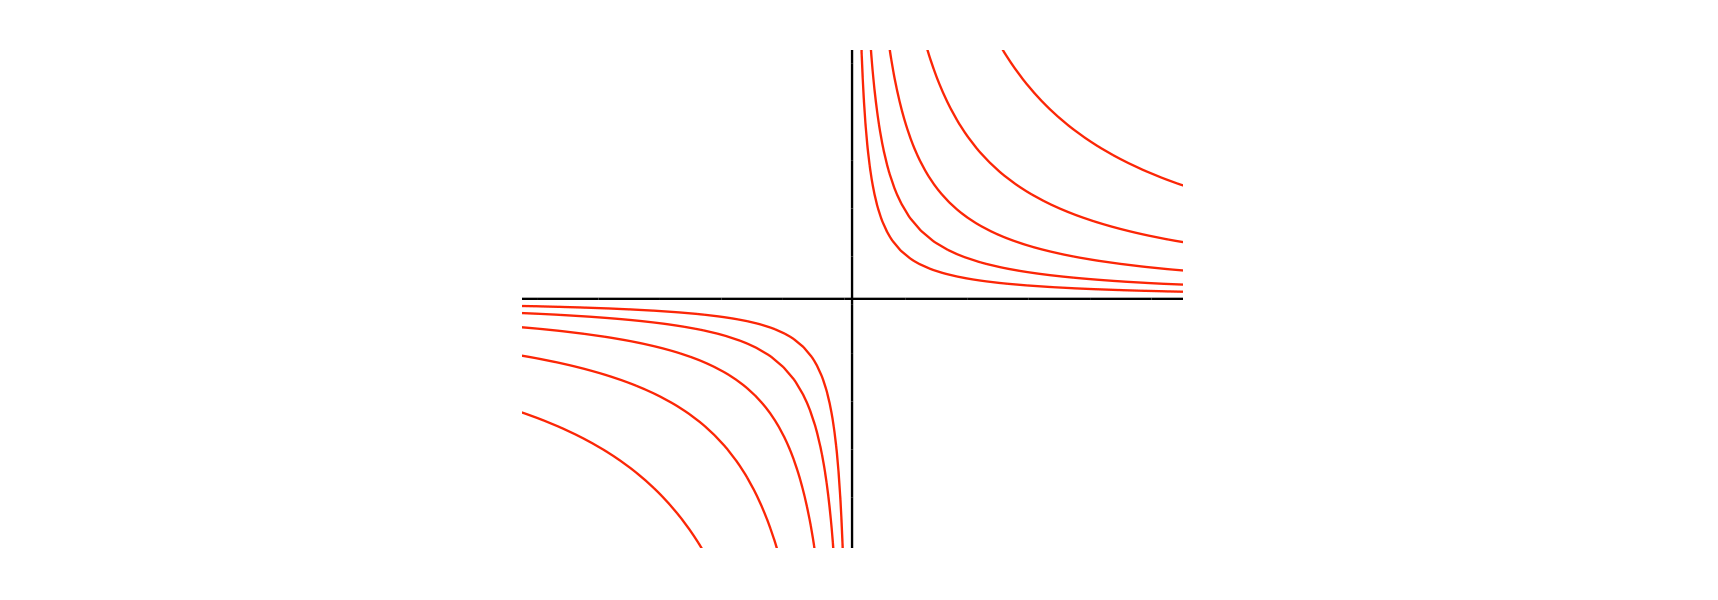
\includegraphics[width=0.62\textwidth]{figure15-1.png}
  \caption{由 $xy=t$ 切出的子空间族；$0$ 处的纤维是由 $xy=0$ 切出的 lci 空间，以黑色显示。（原文 p.~262，Figure 15.1）}
  \label{fig:15-1}
\end{figure}

一旦从光滑过渡到 lci，$T^*X[1]$ 中就出现了新的偶方向。也就是说，由于 $\mathrm{HH}^*$ 现在有对称部分，我们得到了新的非幂零方向。在这个例子中，有一个额外的 $\bA^1$ 从奇点中伸出来，如图 15.2。其想法是：若 $X$ 有奇点，则 $T^*X[1]$ 会在这些奇点上方长出新的偶方向。

\begin{figure}[htbp]
  \centering
  
\includegraphics[width=0.42\textwidth]{figure15-2.png}
  \caption{图 15.1 所述 lci 空间的 $1$-移位余切丛的偶次数部分，在集合论意义下是奇点上方的 $\bA^1$（以红色显示）。（原文 p.~262，Figure 15.2）}
  \label{fig:15-2}
\end{figure}

这对于理解层的自同态很有帮助。但为什么理解层的自同态很重要？关于奇异簇，人们学到的一件事是：$x\in X$ 是光滑点当且仅当 $\cO_x$ 是完美复形，即它有向量丛的有限消解。而具有向量丛的有限消解等价于 $\mathrm{Ext}(\cO_x,\cO_x)$ 是有限维的。% [Tutor Note: 原文此处说 “automorphisms”，但整段讨论的是自同态（endomorphisms）$\mathrm{Ext}(\cO_x,\cO_x)$，且下文正是用 $\mathrm{Ext}$ 的无限维性刻画奇点；按上下文 “automorphisms” 应为 “endomorphisms” 的笔误。]

但若取 $\cO_0$ 的 $\mathrm{Ext}$，其中 $0$ 是 $\{xy=0\}$ 的奇点，我们得到
\begin{equation}\tag{15.60}
\mathrm{Ext}^{even}(\cO_0,\cO_0)\simeq k[t],
\end{equation}
其中变量的次数为 $|t|=2$。所以从同调代数的观点看，这个摩天楼层显得非常“无穷”，尽管它只是一个摩天楼层。关键在于：$T^*X[1]$ 中这些新的方向（如图 15.2）正是为了把这一点纳入考虑而构造的。也就是说，这个 $\mathrm{Ext}$ 恰好看起来就像 $T^*X[1]$ 中粘上的那个 $\bA^1$：
\begin{equation}\tag{15.61}
k[t]=\cO(\bA^1).
\end{equation}
用 Arinkin--Gaitsgory 的凝聚奇异支撑理论来说，$0$ 处摩天楼层的奇异支撑就是这个整个 $\bA^1$：
\begin{equation}\tag{15.62}
\mathrm{SingSupp}(\cO_0)=\bA^1.
\end{equation}
一般地，对任意凝聚层 $\cF$，可以定义（锥形）子集
\begin{equation}\tag{15.63}
\mathrm{SingSupp}(\cF)\subset T^*X[1].
\end{equation}
$\cF$ 是完美的（例如向量丛）当且仅当
\begin{equation}\tag{15.64}
\mathrm{SingSupp}(\cF)=X\hookrightarrow T^*X[1].
\end{equation}
所以奇异支撑给了我们区分有趣的凝聚层与“仅仅是向量丛”的层的方法。

\begin{srcex}{111}
设 $C$ 是亏格为 $g$ 的紧 Riemann 面，$G^\vee$ 是代数群。回想 $\Loc_{G^\vee}(C)$ 是几何 Langlands 的 $B$-侧研究的主要对象。事实证明，这个空间是 lci 的。回顾其定义为
\begin{equation}\tag{15.65}
\Loc_{G^\vee}(C):=\{\pi_1(C)\to G^\vee\}/G^\vee.
\end{equation}
映射 $\pi_1(C)\to G^\vee$ 构成的空间由纤维给出：
\begin{equation}\tag{15.66}
\begin{array}{ccc}
\{\pi_1\to G^\vee\} & \longrightarrow & (G^\vee)^{2g}\\[2pt]
\downarrow & & \downarrow{\scriptstyle \Pi_{[,]}}\\[-2pt]
1 & \longrightarrow & G^\vee
\end{array}
\end{equation}
现在我们可以处处对 $G^\vee$ 取商，得到 $\Loc_{G^\vee}$。也就是说，局部系统的空间由 $(G^\vee)^{2g}$ 经一个方程切出（模同时共轭）。这意味着 $\Loc_{G^\vee}(C)$ 上的层有很好的奇异支撑理论。
\end{srcex}
% [Tutor Note: 这里“一个方程”指 $2g$ 个元素之积的换位子等于 $1$；图中竖直箭头 $\Pi_{[,]}$ 表示把 $(g_1,\dots,g_{2g})$ 送到换位子 $\prod_i[g_i,g_{i+1}]$。$\Loc_{G^\vee}(C)$ 的 lci 性正是指它由这个截面在单位元处的纤维给出。]

于是我们发现：若考虑几何 Langlands 的 $B$-侧，则曲面 $C$ 上的四维理论 $B_{G^\vee}$（即二维理论 $B_{G^\vee}(C\times(-))$）等价于 $\Loc_{G^\vee}(C)$ 上的 $B$-模型。

回想 $B$-模型的可观测量由 $\mathrm{HH}^*$ 给出，而它产生了 $T^*X[1]$。所以 $B$-模型的状态是 $T^*X[1]$ 的某种几何量子化。换句话说，仅仅给定 $T^*X[1]$，要产生范畴 $D^b\mathrm{Coh}(X)$ 是困难的：这正是“艺术”所在。\footnote{Ludwig Faddeev 曾说：“quantization is an art, not a science.”}

\begin{srcrem}{112}
一般的拉格朗日场论必定与这幅量子化图景有关，但在 $A$-侧一切都微妙得多。这是人生经验的一个例子：$B$-侧的事情容易得多；$B$-侧为 $A$-侧的问题提供答案。在 $A$-侧我们处理局部常值映射，即拓扑；在 $B$-侧，映射不是局部常值的，而是代数或全纯映射。
\end{srcrem}
